
Manually assigning topics can be an error-prone activity that can lead to
wrongly specified tags. Literature is plenty of several approaches that mine and exploit available data to analyze repositories. Nevertheless, few of them cope with the topic recommendation task, which can be crucial in the project's development initial phase. Figure \ref{fig:spark} shows an example repository with related topics. By this simple snapshot, a \GH user can figure out that the \emph{apache spark} project makes usage of several programming languages such as \emph{java, r,} and \emph{python} to analyze \emph{big-data} and databases by exploiting common techniques used in this domain \ie \emph{sql and jdbc}. 

\begin{figure*}[h!]
	\centering
	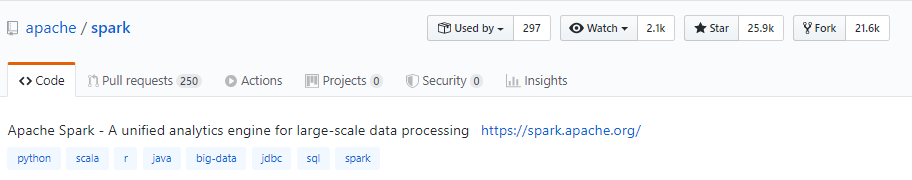
\includegraphics[width=0.8\linewidth]{figs/spark_topics.png}
	\caption{Example of a \GH repository and its topics.}% [??Rename Similarity Computation with Similarity Calculator]
	\label{fig:spark}
\end{figure*}

As mentioned before, the \MNB using the \RM file of a repository to predict featured topics. It involves all the standard techniques employed in the ML domain \ie textual engineering, feature extraction, and training phase. By relying on the multinomial probability distribution, the approach is able to extract relevant information from the \RM file and suggest a set of topics. 

\begin{table}[h]
\centering

\resizebox{8.5cm}{!} {

\begin{tabular}{| p{3.2cm} | p{3.2cm} | }
\hline
 \textbf{Actual Topics} &\textbf{ Predicted topics} \\ \hline
     python,blender-scripts, spaceship, procedural-generation, game-development, 3d        &  
  shell, terminal, \textbf{3d},	opengl,	\textbf{python}        \\ \hline

\end{tabular}
}
\caption{Example of the \MNB outcomes.}
\label{tab:example}
\end{table} 